\documentclass[10pt,onecolumn]{article}
\usepackage[utf8]{inputenc}
\usepackage[english]{babel}
\usepackage[T1]{fontenc}
\usepackage{lmodern}
\usepackage{multicol}
\usepackage{amsmath}
\usepackage{amssymb}
\usepackage{mathrsfs}
\usepackage{graphicx}
\usepackage[margin=1cm]{geometry}

\DeclareMathSizes{10}{10}{10}{10}

% --- 
% Beginning of document
% ---
\begin{document}
{\setlength{\parindent}{0cm}

\part{Definition of the Trig function}

% --- 
% Right triangle definition
% ---
\section{ Right triangle definition}

For this definition we assume that :
\(0 < \theta < \frac{\pi}{2}\) or \(0^{\circ} < \theta < 90^{\circ} \) \\
\begin{tabular}{c|c}
SOH = \(\sin \theta = \frac{opposite}{hypotenuse}\) & \(\csc \theta = \frac{hypotenuse}{opposite}\)  \\
CAH = \(\cos \theta = \frac{adjacent}{hypotenuse}\) & \(\sec \theta = \frac{hypotenuse}{adjacent}\) \\
TOA = \(\tan \theta = \frac{opposite}{adjacent}\) & \(\cot \theta = \frac{adjacent}{opposite}\)  \\
\end{tabular}
% --- 
% Unit circle definition
% ---
\section{Unit circle definition}

For this definition \(\theta\) is any angle.  \\

\begin{tabular}{c|c}
\(\sin \theta = \frac{y}{1} = y \)  & \(\csc \theta = \frac{1}{y} \) \\
\(\cos \theta = \frac{x}{1} = x \) & \(\sec \theta = \frac{1}{x}\) \\
\(\tan \theta = \frac{y}{x} \) & \(\cot \theta = \frac{x}{y}\) \\
\end{tabular}

\part{Basic Properties \& Facts}

% --- 
% Domain
% ---
\section{Domain}

The Domain in all the values of \(\theta\) that can be plugged into the function. \\
\begin{tabular}{c|c}
\(\sin \theta, \theta\)  can be any angle & \(\csc \theta, \theta \neq n\pi, n = 0, \pm 1, \pm 2, ... \)\\
\(\cos \theta, \theta\)  can be any angle & \(\sec \theta, \theta \neq (n + \frac{1}{2})\pi, n = 0, \pm 1, \pm 2, ... \) \\
\(\tan \theta, \theta \neq (n + \frac{1}{2})\pi, n = 0, \pm 1, \pm 2, ...\) & \(\cot \theta, \theta \neq n\pi, n = 0, \pm 1, \pm 2, ... \) \\
\end{tabular}
% --- 
% Range
% ---
\section{Range}

The range is all possible values to get out of the function. \\

\begin{tabular}{c|c}
\(-1 \le \sin \theta \le 1\) & \(\csc \theta \ge 1\) and \(\csc \theta \le -1\) \\
\(-1 \le \cos \theta \le 1\) & \(\sec \theta \ge 1\) and \(\sec \theta \le -1\) \\
\(-\infty \le \tan\theta \le \infty\) & \(-\infty \le \cot \theta \le \infty\) \\
\end{tabular}

% --- 
% Period
% ---
\section{Period}

The period of a function is the number, T, such that \(f(\theta + T) = f(\theta) \). \\ 
So if \(w\) is a fixed number and \(\theta\) is any angle we have the following periods.

\begin{tabular}{c|c}
\(\sin(w\theta) \rightarrow T = \frac{2\pi}{w} \) & \(\csc(w\theta) \rightarrow T = \frac{2\pi}{w} \) \\
\(\cos(w\theta) \rightarrow T = \frac{2\pi}{w} \) & \(\sec(w\theta) \rightarrow T = \frac{2\pi}{w} \) \\
\(\tan(w\theta) \rightarrow T = \frac{\pi}{w} \) & \(\cot(w\theta) \rightarrow T = \frac{\pi}{w} \)\\
\end{tabular}
\pagebreak

\part{Formulas and Identities}

% --- 
% Tangent and Cotangent Identities
% ---
\section{Tangent and Cotangent Identities}


\(\tan \theta = \frac{\sin \theta}{\cos \theta}\) \\
\(\cot \theta = \frac{\cos \theta}{\sin \theta}\) \\

% --- 
% Reciprocal Identities
% ---
\section{Reciprocal Identities}
\begin{tabular}{c|c}
\(\csc \theta = \frac{1}{\sin \theta}\) & \(\sin \theta = \frac{1}{\csc \theta}\) \\
\(\sec \theta = \frac{1}{\cos \theta}\) & \(\cos \theta = \frac{1}{\sec \theta}\)\\
\(\cot \theta = \frac{1}{\tan \theta}\) & \(\tan \theta = \frac{1}{\cot \theta}\) \\
\end{tabular}

% --- 
% Pythagorean  Identities
% ---
\section{Pythagorean  Identities}

\(\sin^2 \theta + \cos^2 \theta = 1 \) \\
\(\tan^2 \theta + 1 = \sec^2 \theta \) \\
\(1 + \cot^2 \theta = \csc^2 \theta \) \\



% --- 
% Even/Odd Identities
% ---
\section{Even/Odd Identities}
\begin{tabular}{c|c}
\(\sin(-\theta) = -\sin \theta\) & \(\csc(-\theta) = -\csc \theta\) \\
\(\cos(-\theta) = \cos \theta\) & \(\sec(-\theta) = \sec \theta\) \\
\(\tan(-\theta) = -\tan \theta\) &\(\cot(-\theta) = -\cot \theta\) \\
\end{tabular}


% --- 
%Periodic Formulas
% ---
\section{Periodic Formulas}
If n is integer.
\begin{tabular}{c|c}
\(\sin(\theta + 2\pi n) = \sin \theta\) & \(\csc(\theta + 2\pi n) = \csc \theta\)\\
\(\cos(\theta + 2\pi n) = \cos \theta\) & \(\sec(\theta + 2\pi n) = \sec \theta\)\\
\(\tan(\theta + \pi n) = \tan \theta\) & \(\cot(\theta + \pi n) = \cot \theta\) \\
\end{tabular}


% --- 
% Double Angle Formulas
% ---
\section{Double Angle Formulas}

\(\sin(2\theta) = 2\sin \theta \cos \theta\) \\
\(\cos(2\theta) = 2\cos^2 \theta - \sin^2 \theta = 2\cos^2 \theta - 1 = 1 - 2\sin^2 \theta\) \\
\(\tan(2\theta) = \frac{2\tan \theta}{1 - \tan^2 \theta}\) \\

% --- 
%Degrees to Radians Formulas
% ---
\section{Degrees to Radians Formulas}

If x is an angle in degrees and t is an angle in radians then \\
\(\frac{\pi}{180} = \frac{t}{x} \Rightarrow t = \frac{\pi x}{180} and x = \frac{180t}{\pi}\) \\

% --- 
% Half Angle Formulas
% ---
\section{Half Angle Formulas}

\(\sin^2 \theta = \frac{1 - \cos(2\theta)}{2}\) \\
\(\cos^2 \theta = \frac{1 + \cos(2\theta)}{2}\) \\
\(\tan^2 \theta = \frac{1 - \cos(2\theta)}{1 + cos(2\theta)}\) \\

% --- 
%Sum and Difference Formulas
% ---
\section{Sum and Difference Formulas}

\(\sin(\alpha \pm \beta) = \sin \alpha \cos \beta \pm \cos \alpha \sin \beta \) \\
\(\cos(\alpha \pm \beta) = \cos \alpha \cos \beta \mp \sin \alpha \sin \beta \) \\
\(\tan(\alpha \pm \beta) = \frac{\tan \alpha \pm \tan \beta}{1 \mp \tan \alpha \tan \beta} \) \\

% --- 
%Product to Sum Formulas
% ---
\section{Product to Sum Formulas}

\(\sin \alpha \sin \beta = \frac{\cos(\alpha - \beta) - \cos(\alpha + \beta)}{2}\) \\
\(\cos \alpha \cos \beta = \frac{\cos(\alpha - \beta) + \cos(\alpha + \beta)}{2}\) \\
\(\sin \alpha \cos \beta = \frac{\sin(\alpha + \beta) + \sin(\alpha - \beta)}{2}\) \\
\(\cos \alpha \sin \beta = \frac{\sin(\alpha + \beta) - \sin(\alpha - \beta)}{2}\) \\

% --- 
% Sum to Product Formulas
% ---
\section{Sum to Product Formulas}

\(\sin \alpha + \sin \beta = 2 \sin (\frac{\alpha + \beta}{2})\cos(\frac{\alpha - \beta}{2})\) \\
\(\sin \alpha - \sin \beta = 2 \cos (\frac{\alpha + \beta}{2})\sin(\frac{\alpha - \beta}{2})\) \\
\(\cos \alpha + \cos \beta = 2 \cos (\frac{\alpha + \beta}{2})\cos(\frac{\alpha - \beta}{2})\) \\
\(\cos \alpha - \cos \beta = -2 \sin (\frac{\alpha + \beta}{2})\sin(\frac{\alpha - \beta}{2})\) \\


% --- 
% Cofunction  Formulas
% ---
\section{Cofunction Formulas}

\begin{tabular}{c|c}
\(\sin(\frac{\pi}{2} - \theta) = \cos \theta\) & \(\cos(\frac{\pi}{2} - \theta) = \sin \theta\)\\
\(\csc(\frac{\pi}{2} - \theta) = \sec \theta\) & \(\sec(\frac{\pi}{2} - \theta) = \csc \theta\)\\
\(\tan(\frac{\pi}{2} - \theta) = \cot \theta\) & \(\cot(\frac{\pi}{2} - \theta) = \tan \theta\) \\
\end{tabular}

\pagebreak

\part{Unit Circle}

\begin{figure}[Unit Circle]
\centering
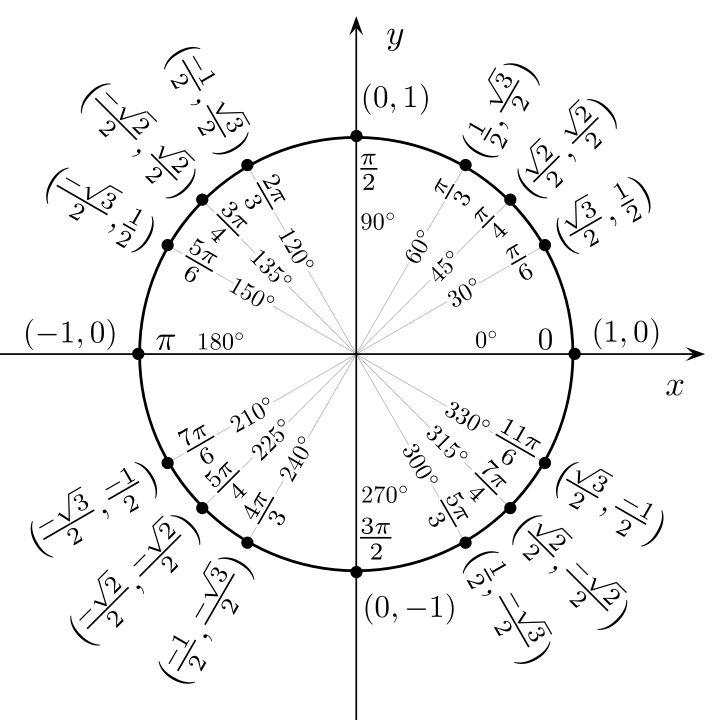
\includegraphics[width=90mm]{unit_circle.png}
\caption{Unit Circle}
\label{overflow}
\end{figure}

For any ordered pair on the unit circle (x, y) : \(\cos \theta = x\) and \(\sin \theta = y\)

Example :

\(\cos(\frac{5\pi}{3}) = \frac{1}{2}\) \\
\(\sin(\frac{5\pi}{3}) = -\frac{sqrt{3}}{2}\) \\
\pagebreak

\part{Inverse Trig Functions}

% --- 
% Definition 
% ---
\section{Definition }

\(y = \sin^{-1} x\) is equivalent to \(x = \sin y\) \\
\(y = \cos^{-1} x\) is equivalent to \(x = \cos y\) \\
\(y = \tan^{-1} x\) is equivalent to \(x = \tan y\) \\


% --- 
% Domain and Range  Formulas
% ---
\section{ Domain and Range  Formulas}

\begin{tabular}{ccc}
Function & Domain & Range \\
\(y = \sin^{-1} x\) & \(-1 \le x \le 1\) & \(-\frac{\pi}{2} \le y \le \frac{\pi}{2}\) \\
\(y = \cos^{-1} x\) & \(-1 \le x \le 1\) & \(0 \le y \le \pi\) \\
\(y = \tan^{-1} x\) & \(-\infty \le x \le \infty\) & \(-\frac{\pi}{2} \le y \le \frac{\pi}{2}\)
\end{tabular}

% --- 
% Inverse Properties
% ---
\section{Inverse Properties}
\begin{tabular}{c|c}
\(\cos(\cos^{-1}(x)) = x \) & \(\cos^{-1}(\cos(x)) = x \) \\
\(\sin(\sin^{-1}(x)) = x \) & \(\sin^{-1(\sin}(x)) = x \)\\
\(\tan(\tan^{-1}(x)) = x \) & \(\tan^{-1}(\tan(x)) = x \)\\
\end{tabular}

% --- 
% Alternate Notation
% ---
\section{Alternate Notation}

\(\sin^{-1}x = arcsin x \) \\
\(\cos^{-1}x = arccos x \) \\
\(\tan^{-1}x = arctan x \) \\


\part{Law of Sines, Cosines and Tangents}

% --- 
% Law of Sines
% ---
\section{Law of Sines}

\(\frac{\sin \alpha}{a} = \frac{\sin \beta}{b} = \frac{\sin \gamma}{c} \) \\


% --- 
% Law of Cosines
% ---
\section{ Law of Cosines}

\(a^2 = b^2 + c^2 - 2bc\cos \alpha \) \\
\(b^2 = a^2 + c^2 - 2ac\cos \beta \) \\
\(c^2 = a^2 + b^2 - 2ab\cos \gamma \) \\


% --- 
% Mollweide's Formula
% ---
\section{Mollweide's Formula}

\(\frac{a + b}{c} = \frac{\cos \frac{1}{2}(\alpha - \beta)}{\sin \frac{1}{2} \gamma}\) \\


% --- 
% Law of Tangents
% ---
\section{Law of Tangents}

\(\frac{a - b}{a + b} = \frac{\tan \frac{1}{2}(\alpha - \beta)}{\tan \frac{1}{2}(\alpha + \beta)} \) \\
\(\frac{b - c}{b + cb} = \frac{\tan \frac{1}{2}(\beta - \gamma)}{\tan \frac{1}{2}(\beta + \gamma)} \) \\
\(\frac{a - c}{a + c} = \frac{\tan \frac{1}{2}(\alpha - \gamma)}{\tan \frac{1}{2}(\alpha + \gamma)} \) \\



% --- 
% End of document
% ---
\end{document}
